\documentclass[1p]{elsarticle_modified}
%\bibliographystyle{elsarticle-num}

%\usepackage[colorlinks]{hyperref}
%\usepackage{abbrmath_seonhwa} %\Abb, \Ascr, \Acal ,\Abf, \Afrak
\usepackage{amsfonts}
\usepackage{amssymb}
\usepackage{amsmath}
\usepackage{amsthm}
\usepackage{scalefnt}
\usepackage{amsbsy}
\usepackage{kotex}
\usepackage{caption}
\usepackage{subfig}
\usepackage{color}
\usepackage{graphicx}
\usepackage{xcolor} %% white, black, red, green, blue, cyan, magenta, yellow
\usepackage{float}
\usepackage{setspace}
\usepackage{hyperref}

\usepackage{tikz}
\usetikzlibrary{arrows}

\usepackage{multirow}
\usepackage{array} % fixed length table
\usepackage{hhline}

%%%%%%%%%%%%%%%%%%%%%
\makeatletter
\renewcommand*\env@matrix[1][\arraystretch]{%
	\edef\arraystretch{#1}%
	\hskip -\arraycolsep
	\let\@ifnextchar\new@ifnextchar
	\array{*\c@MaxMatrixCols c}}
\makeatother %https://tex.stackexchange.com/questions/14071/how-can-i-increase-the-line-spacing-in-a-matrix
%%%%%%%%%%%%%%%

\usepackage[normalem]{ulem}

\newcommand{\msout}[1]{\ifmmode\text{\sout{\ensuremath{#1}}}\else\sout{#1}\fi}
%SOURCE: \msout is \stkout macro in https://tex.stackexchange.com/questions/20609/strikeout-in-math-mode

\newcommand{\cancel}[1]{
	\ifmmode
	{\color{red}\msout{#1}}
	\else
	{\color{red}\sout{#1}}
	\fi
}

\newcommand{\add}[1]{
	{\color{blue}\uwave{#1}}
}

\newcommand{\replace}[2]{
	\ifmmode
	{\color{red}\msout{#1}}{\color{blue}\uwave{#2}}
	\else
	{\color{red}\sout{#1}}{\color{blue}\uwave{#2}}
	\fi
}

\newcommand{\Sol}{\mathcal{S}} %segment
\newcommand{\D}{D} %diagram
\newcommand{\A}{\mathcal{A}} %arc


%%%%%%%%%%%%%%%%%%%%%%%%%%%%%5 test

\def\sl{\operatorname{\textup{SL}}(2,\Cbb)}
\def\psl{\operatorname{\textup{PSL}}(2,\Cbb)}
\def\quan{\mkern 1mu \triangleright \mkern 1mu}

\theoremstyle{definition}
\newtheorem{thm}{Theorem}[section]
\newtheorem{prop}[thm]{Proposition}
\newtheorem{lem}[thm]{Lemma}
\newtheorem{ques}[thm]{Question}
\newtheorem{cor}[thm]{Corollary}
\newtheorem{defn}[thm]{Definition}
\newtheorem{exam}[thm]{Example}
\newtheorem{rmk}[thm]{Remark}
\newtheorem{alg}[thm]{Algorithm}

\newcommand{\I}{\sqrt{-1}}
\begin{document}

%\begin{frontmatter}
%
%\title{Boundary parabolic representations of knots up to 8 crossings}
%
%%% Group authors per affiliation:
%\author{Yunhi Cho} 
%\address{Department of Mathematics, University of Seoul, Seoul, Korea}
%\ead{yhcho@uos.ac.kr}
%
%
%\author{Seonhwa Kim} %\fnref{s_kim}}
%\address{Center for Geometry and Physics, Institute for Basic Science, Pohang, 37673, Korea}
%\ead{ryeona17@ibs.re.kr}
%
%\author{Hyuk Kim}
%\address{Department of Mathematical Sciences, Seoul National University, Seoul 08826, Korea}
%\ead{hyukkim@snu.ac.kr}
%
%\author{Seokbeom Yoon}
%\address{Department of Mathematical Sciences, Seoul National University, Seoul, 08826,  Korea}
%\ead{sbyoon15@snu.ac.kr}
%
%\begin{abstract}
%We find all boundary parabolic representation of knots up to 8 crossings.
%
%\end{abstract}
%\begin{keyword}
%    \MSC[2010] 57M25 
%\end{keyword}
%
%\end{frontmatter}

%\linenumbers
%\tableofcontents
%
\newcommand\colored[1]{\textcolor{white}{\rule[-0.35ex]{0.8em}{1.4ex}}\kern-0.8em\color{red} #1}%
%\newcommand\colored[1]{\textcolor{white}{ #1}\kern-2.17ex	\textcolor{white}{ #1}\kern-1.81ex	\textcolor{white}{ #1}\kern-2.15ex\color{red}#1	}

{\Large $\underline{12a_{1253}~(K12a_{1253})}$}

\setlength{\tabcolsep}{10pt}
\renewcommand{\arraystretch}{1.6}
\vspace{1cm}\begin{tabular}{m{100pt}>{\centering\arraybackslash}m{274pt}}
\multirow{5}{120pt}{
	\centering
	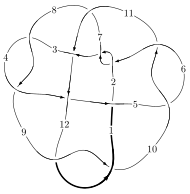
\includegraphics[width=112pt]{../../../GIT/diagram.site/Diagrams/png/2054_12a_1253.png}\\
\ \ \ A knot diagram\footnotemark}&
\allowdisplaybreaks
\textbf{Linearized knot diagam} \\
\cline{2-2}
 &
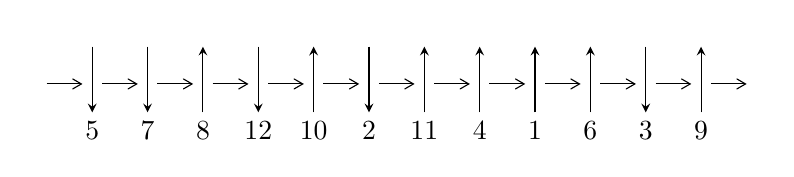
\begin{tikzpicture}[x=20pt, y=17pt]
	% nodes
	\node (C0) at (0, 0) {};
	\node (C1) at (1, 0) {};
	\node (C1U) at (1, +1) {};
	\node (C1D) at (1, -1) {5};

	\node (C2) at (2, 0) {};
	\node (C2U) at (2, +1) {};
	\node (C2D) at (2, -1) {7};

	\node (C3) at (3, 0) {};
	\node (C3U) at (3, +1) {};
	\node (C3D) at (3, -1) {8};

	\node (C4) at (4, 0) {};
	\node (C4U) at (4, +1) {};
	\node (C4D) at (4, -1) {12};

	\node (C5) at (5, 0) {};
	\node (C5U) at (5, +1) {};
	\node (C5D) at (5, -1) {10};

	\node (C6) at (6, 0) {};
	\node (C6U) at (6, +1) {};
	\node (C6D) at (6, -1) {2};

	\node (C7) at (7, 0) {};
	\node (C7U) at (7, +1) {};
	\node (C7D) at (7, -1) {11};

	\node (C8) at (8, 0) {};
	\node (C8U) at (8, +1) {};
	\node (C8D) at (8, -1) {4};

	\node (C9) at (9, 0) {};
	\node (C9U) at (9, +1) {};
	\node (C9D) at (9, -1) {1};

	\node (C10) at (10, 0) {};
	\node (C10U) at (10, +1) {};
	\node (C10D) at (10, -1) {6};

	\node (C11) at (11, 0) {};
	\node (C11U) at (11, +1) {};
	\node (C11D) at (11, -1) {3};

	\node (C12) at (12, 0) {};
	\node (C12U) at (12, +1) {};
	\node (C12D) at (12, -1) {9};
	\node (C13) at (13, 0) {};

	% arrows
	\draw[->,>={angle 60}]
	(C0) edge (C1) (C1) edge (C2) (C2) edge (C3) (C3) edge (C4) (C4) edge (C5) (C5) edge (C6) (C6) edge (C7) (C7) edge (C8) (C8) edge (C9) (C9) edge (C10) (C10) edge (C11) (C11) edge (C12) (C12) edge (C13) ;	\draw[->,>=stealth]
	(C1U) edge (C1D) (C2U) edge (C2D) (C3D) edge (C3U) (C4U) edge (C4D) (C5D) edge (C5U) (C6U) edge (C6D) (C7D) edge (C7U) (C8D) edge (C8U) (C9D) edge (C9U) (C10D) edge (C10U) (C11U) edge (C11D) (C12D) edge (C12U) ;
	\end{tikzpicture} \\
\hhline{~~} \\& 
\textbf{Solving Sequence} \\ \cline{2-2} 
 &
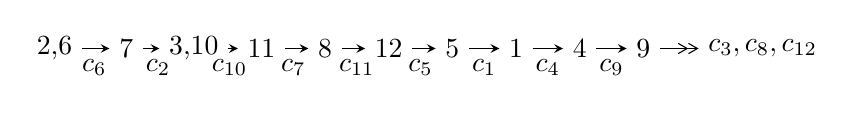
\begin{tikzpicture}[x=23pt, y=7pt]
	% node
	\node (A0) at (-1/8, 0) {2,6};
	\node (A1) at (1, 0) {7};
	\node (A2) at (33/16, 0) {3,10};
	\node (A3) at (25/8, 0) {11};
	\node (A4) at (33/8, 0) {8};
	\node (A5) at (41/8, 0) {12};
	\node (A6) at (49/8, 0) {5};
	\node (A7) at (57/8, 0) {1};
	\node (A8) at (65/8, 0) {4};
	\node (A9) at (73/8, 0) {9};
	\node (C1) at (1/2, -1) {$c_{6}$};
	\node (C2) at (3/2, -1) {$c_{2}$};
	\node (C3) at (21/8, -1) {$c_{10}$};
	\node (C4) at (29/8, -1) {$c_{7}$};
	\node (C5) at (37/8, -1) {$c_{11}$};
	\node (C6) at (45/8, -1) {$c_{5}$};
	\node (C7) at (53/8, -1) {$c_{1}$};
	\node (C8) at (61/8, -1) {$c_{4}$};
	\node (C9) at (69/8, -1) {$c_{9}$};
	\node (A10) at (11, 0) {$c_{3},c_{8},c_{12}$};

	% edge
	\draw[->,>=stealth]	
	(A0) edge (A1) (A1) edge (A2) (A2) edge (A3) (A3) edge (A4) (A4) edge (A5) (A5) edge (A6) (A6) edge (A7) (A7) edge (A8) (A8) edge (A9) ;
	\draw[->>,>={angle 60}]	
	(A9) edge (A10);
\end{tikzpicture} \\ 

\end{tabular} \\

\footnotetext{
The image of knot diagram is generated by the software ``\textbf{Draw programme}" developed by Andrew Bartholomew(\url{http://www.layer8.co.uk/maths/draw/index.htm\#Running-draw}), where we modified some parts for our purpose(\url{https://github.com/CATsTAILs/LinksPainter}).
}\phantom \\ \newline 
\centering \textbf{Ideals for irreducible components\footnotemark of $X_{\text{par}}$} 
 
\begin{align*}
I^u_{1}&=\langle 
-1.59766\times10^{581} u^{124}+3.43383\times10^{581} u^{123}+\cdots+2.82859\times10^{581} b+5.30736\times10^{583},\\
\phantom{I^u_{1}}&\phantom{= \langle  }2.20394\times10^{582} u^{124}-4.77048\times10^{582} u^{123}+\cdots+4.80860\times10^{582} a-7.41864\times10^{584},\\
\phantom{I^u_{1}}&\phantom{= \langle  }u^{125}-3 u^{124}+\cdots-1955 u+289\rangle \\
I^u_{2}&=\langle 
791694037 u^{18}+148281897 u^{17}+\cdots+2256529259 b+2264697959,\\
\phantom{I^u_{2}}&\phantom{= \langle  }-162403155 u^{18}+758589616 u^{17}+\cdots+2256529259 a+24533522042,\\
\phantom{I^u_{2}}&\phantom{= \langle  }u^{19}-8 u^{17}+\cdots-15 u+1\rangle \\
I^u_{3}&=\langle 
b+1,\;a,\;u^2- u-1\rangle \\
I^u_{4}&=\langle 
b+1,\;a-1,\;u+1\rangle \\
\\
\end{align*}
\raggedright * 4 irreducible components of $\dim_{\mathbb{C}}=0$, with total 147 representations.\\
\footnotetext{All coefficients of polynomials are rational numbers. But the coefficients are sometimes approximated in decimal forms when there is not enough margin.}
\newpage
\renewcommand{\arraystretch}{1}
\centering \section*{I. $I^u_{1}= \langle -1.60\times10^{581} u^{124}+3.43\times10^{581} u^{123}+\cdots+2.83\times10^{581} b+5.31\times10^{583},\;2.20\times10^{582} u^{124}-4.77\times10^{582} u^{123}+\cdots+4.81\times10^{582} a-7.42\times10^{584},\;u^{125}-3 u^{124}+\cdots-1955 u+289 \rangle$}
\flushleft \textbf{(i) Arc colorings}\\
\begin{tabular}{m{7pt} m{180pt} m{7pt} m{180pt} }
\flushright $a_{2}=$&$\begin{pmatrix}0\\u\end{pmatrix}$ \\
\flushright $a_{6}=$&$\begin{pmatrix}1\\0\end{pmatrix}$ \\
\flushright $a_{7}=$&$\begin{pmatrix}1\\u^2\end{pmatrix}$ \\
\flushright $a_{3}=$&$\begin{pmatrix}- u\\- u^3+u\end{pmatrix}$ \\
\flushright $a_{10}=$&$\begin{pmatrix}-0.458334 u^{124}+0.992072 u^{123}+\cdots-817.690 u+154.278\\0.564827 u^{124}-1.21397 u^{123}+\cdots+1047.83 u-187.633\end{pmatrix}$ \\
\flushright $a_{11}=$&$\begin{pmatrix}0.106493 u^{124}-0.221902 u^{123}+\cdots+230.141 u-33.3541\\0.564827 u^{124}-1.21397 u^{123}+\cdots+1047.83 u-187.633\end{pmatrix}$ \\
\flushright $a_{8}=$&$\begin{pmatrix}0.371742 u^{124}-0.828981 u^{123}+\cdots+745.819 u-139.719\\-0.191219 u^{124}+0.426785 u^{123}+\cdots-403.224 u+74.5168\end{pmatrix}$ \\
\flushright $a_{12}=$&$\begin{pmatrix}-0.321539 u^{124}+0.694405 u^{123}+\cdots-558.595 u+107.776\\0.666292 u^{124}-1.43070 u^{123}+\cdots+1241.24 u-222.472\end{pmatrix}$ \\
\flushright $a_{5}=$&$\begin{pmatrix}-0.280445 u^{124}+0.624569 u^{123}+\cdots-586.063 u+112.854\\-0.311341 u^{124}+0.691375 u^{123}+\cdots-323.906 u+58.2541\end{pmatrix}$ \\
\flushright $a_{1}=$&$\begin{pmatrix}0.843078 u^{124}-1.84273 u^{123}+\cdots+1707.88 u-304.272\\-0.559460 u^{124}+1.23368 u^{123}+\cdots-1142.91 u+208.255\end{pmatrix}$ \\
\flushright $a_{4}=$&$\begin{pmatrix}-0.650008 u^{124}+1.44187 u^{123}+\cdots-1314.29 u+240.546\\0.415494 u^{124}-0.925040 u^{123}+\cdots+859.265 u-156.839\end{pmatrix}$ \\
\flushright $a_{9}=$&$\begin{pmatrix}0.733999 u^{124}-1.60760 u^{123}+\cdots+1479.66 u-262.978\\-0.615104 u^{124}+1.36954 u^{123}+\cdots-1246.28 u+226.921\end{pmatrix}$\\&\end{tabular}
\flushleft \textbf{(ii) Obstruction class $= -1$}\\~\\
\flushleft \textbf{(iii) Cusp Shapes $= 2.20245 u^{124}-2.27856 u^{123}+\cdots+8267.63 u-1316.86$}\\~\\
\newpage\renewcommand{\arraystretch}{1}
\flushleft \textbf{(iv) u-Polynomials at the component}\newline \\
\begin{tabular}{m{50pt}|m{274pt}}
Crossings & \hspace{64pt}u-Polynomials at each crossing \\
\hline $$\begin{aligned}c_{1}\end{aligned}$$&$\begin{aligned}
&u^{125}+6 u^{124}+\cdots-103752 u+326
\end{aligned}$\\
\hline $$\begin{aligned}c_{2},c_{6}\end{aligned}$$&$\begin{aligned}
&u^{125}-3 u^{124}+\cdots-1955 u+289
\end{aligned}$\\
\hline $$\begin{aligned}c_{3},c_{8}\end{aligned}$$&$\begin{aligned}
&u^{125}-49 u^{123}+\cdots+1952 u-64
\end{aligned}$\\
\hline $$\begin{aligned}c_{4}\end{aligned}$$&$\begin{aligned}
&u^{125}+11 u^{124}+\cdots+5083935 u+755075
\end{aligned}$\\
\hline $$\begin{aligned}c_{5},c_{10}\end{aligned}$$&$\begin{aligned}
&u^{125}+15 u^{124}+\cdots+1470 u+223
\end{aligned}$\\
\hline $$\begin{aligned}c_{7}\end{aligned}$$&$\begin{aligned}
&u^{125}-3 u^{124}+\cdots-1329 u-1097
\end{aligned}$\\
\hline $$\begin{aligned}c_{9},c_{12}\end{aligned}$$&$\begin{aligned}
&u^{125}+2 u^{124}+\cdots-3 u+1
\end{aligned}$\\
\hline $$\begin{aligned}c_{11}\end{aligned}$$&$\begin{aligned}
&u^{125}+11 u^{124}+\cdots-19 u+1
\end{aligned}$\\
\hline
\end{tabular}\\~\\
\newpage\renewcommand{\arraystretch}{1}
\flushleft \textbf{(v) Riley Polynomials at the component}\newline \\
\begin{tabular}{m{50pt}|m{274pt}}
Crossings & \hspace{64pt}Riley Polynomials at each crossing \\
\hline $$\begin{aligned}c_{1}\end{aligned}$$&$\begin{aligned}
&y^{125}+26 y^{124}+\cdots+11898756036 y-106276
\end{aligned}$\\
\hline $$\begin{aligned}c_{2},c_{6}\end{aligned}$$&$\begin{aligned}
&y^{125}-85 y^{124}+\cdots-9039053 y-83521
\end{aligned}$\\
\hline $$\begin{aligned}c_{3},c_{8}\end{aligned}$$&$\begin{aligned}
&y^{125}-98 y^{124}+\cdots+891904 y-4096
\end{aligned}$\\
\hline $$\begin{aligned}c_{4}\end{aligned}$$&$\begin{aligned}
&y^{125}-51 y^{124}+\cdots-11330459493975 y-570138255625
\end{aligned}$\\
\hline $$\begin{aligned}c_{5},c_{10}\end{aligned}$$&$\begin{aligned}
&y^{125}-179 y^{124}+\cdots+4984526 y-49729
\end{aligned}$\\
\hline $$\begin{aligned}c_{7}\end{aligned}$$&$\begin{aligned}
&y^{125}-23 y^{124}+\cdots+199287673 y-1203409
\end{aligned}$\\
\hline $$\begin{aligned}c_{9},c_{12}\end{aligned}$$&$\begin{aligned}
&y^{125}-106 y^{124}+\cdots-155 y-1
\end{aligned}$\\
\hline $$\begin{aligned}c_{11}\end{aligned}$$&$\begin{aligned}
&y^{125}-99 y^{124}+\cdots+589 y-1
\end{aligned}$\\
\hline
\end{tabular}\\~\\
\newpage\flushleft \textbf{(vi) Complex Volumes and Cusp Shapes}
$$\begin{array}{c|c|c}  
\text{Solutions to }I^u_{1}& \I (\text{vol} + \sqrt{-1}CS) & \text{Cusp shape}\\
 \hline 
\begin{aligned}
u &= \phantom{-}0.942487 + 0.335420 I \\
a &= -1.31065 - 0.55928 I \\
b &= \phantom{-}0.949578 - 0.100314 I\end{aligned}
 & \phantom{-}1.073150 - 0.413455 I & \phantom{-0.000000 } 0 \\ \hline\begin{aligned}
u &= \phantom{-}0.942487 - 0.335420 I \\
a &= -1.31065 + 0.55928 I \\
b &= \phantom{-}0.949578 + 0.100314 I\end{aligned}
 & \phantom{-}1.073150 + 0.413455 I & \phantom{-0.000000 } 0 \\ \hline\begin{aligned}
u &= -0.998836\phantom{ +0.000000I} \\
a &= \phantom{-}0.104757\phantom{ +0.000000I} \\
b &= -8.54734\phantom{ +0.000000I}\end{aligned}
 & -0.00222811\phantom{ +0.000000I} & \phantom{-0.000000 } 0 \\ \hline\begin{aligned}
u &= -0.984421 + 0.123698 I \\
a &= \phantom{-}1.85676 - 1.50641 I \\
b &= -1.338110 - 0.348323 I\end{aligned}
 & \phantom{-}2.57285 + 3.74721 I & \phantom{-0.000000 } 0 \\ \hline\begin{aligned}
u &= -0.984421 - 0.123698 I \\
a &= \phantom{-}1.85676 + 1.50641 I \\
b &= -1.338110 + 0.348323 I\end{aligned}
 & \phantom{-}2.57285 - 3.74721 I & \phantom{-0.000000 } 0 \\ \hline\begin{aligned}
u &= -1.006450 + 0.082045 I \\
a &= -1.41830 + 0.84737 I \\
b &= \phantom{-}1.243520 + 0.340332 I\end{aligned}
 & -2.02666 + 1.11572 I & \phantom{-0.000000 } 0 \\ \hline\begin{aligned}
u &= -1.006450 - 0.082045 I \\
a &= -1.41830 - 0.84737 I \\
b &= \phantom{-}1.243520 - 0.340332 I\end{aligned}
 & -2.02666 - 1.11572 I & \phantom{-0.000000 } 0 \\ \hline\begin{aligned}
u &= \phantom{-}0.969937 + 0.142867 I \\
a &= -0.025056 - 0.679227 I \\
b &= -0.92183 - 1.61532 I\end{aligned}
 & \phantom{-}4.14076 + 0.37848 I & \phantom{-0.000000 } 0 \\ \hline\begin{aligned}
u &= \phantom{-}0.969937 - 0.142867 I \\
a &= -0.025056 + 0.679227 I \\
b &= -0.92183 + 1.61532 I\end{aligned}
 & \phantom{-}4.14076 - 0.37848 I & \phantom{-0.000000 } 0 \\ \hline\begin{aligned}
u &= \phantom{-}0.999678 + 0.255939 I \\
a &= -0.295500 - 0.549772 I \\
b &= \phantom{-}1.33355 - 0.68586 I\end{aligned}
 & \phantom{-}3.57785 - 0.70217 I & \phantom{-0.000000 } 0\\
 \hline 
 \end{array}$$\newpage$$\begin{array}{c|c|c}  
\text{Solutions to }I^u_{1}& \I (\text{vol} + \sqrt{-1}CS) & \text{Cusp shape}\\
 \hline 
\begin{aligned}
u &= \phantom{-}0.999678 - 0.255939 I \\
a &= -0.295500 + 0.549772 I \\
b &= \phantom{-}1.33355 + 0.68586 I\end{aligned}
 & \phantom{-}3.57785 + 0.70217 I & \phantom{-0.000000 } 0 \\ \hline\begin{aligned}
u &= -0.728834 + 0.747827 I \\
a &= -1.39852 + 0.79835 I \\
b &= \phantom{-}0.993598 + 0.529369 I\end{aligned}
 & \phantom{-}3.46231 + 3.84978 I & \phantom{-0.000000 } 0 \\ \hline\begin{aligned}
u &= -0.728834 - 0.747827 I \\
a &= -1.39852 - 0.79835 I \\
b &= \phantom{-}0.993598 - 0.529369 I\end{aligned}
 & \phantom{-}3.46231 - 3.84978 I & \phantom{-0.000000 } 0 \\ \hline\begin{aligned}
u &= \phantom{-}0.947940\phantom{ +0.000000I} \\
a &= \phantom{-}0.411989\phantom{ +0.000000I} \\
b &= -3.26607\phantom{ +0.000000I}\end{aligned}
 & \phantom{-}4.49095\phantom{ +0.000000I} & \phantom{-0.000000 } 0 \\ \hline\begin{aligned}
u &= -0.201015 + 0.900653 I \\
a &= -2.01584 - 0.72120 I \\
b &= \phantom{-}1.41913 + 0.13506 I\end{aligned}
 & \phantom{-}11.14340 - 2.83478 I & \phantom{-0.000000 } 0 \\ \hline\begin{aligned}
u &= -0.201015 - 0.900653 I \\
a &= -2.01584 + 0.72120 I \\
b &= \phantom{-}1.41913 - 0.13506 I\end{aligned}
 & \phantom{-}11.14340 + 2.83478 I & \phantom{-0.000000 } 0 \\ \hline\begin{aligned}
u &= \phantom{-}0.763397 + 0.778071 I \\
a &= \phantom{-}0.764289 - 0.538999 I \\
b &= -0.245655 + 0.161369 I\end{aligned}
 & \phantom{-}5.66067 + 3.97448 I & \phantom{-0.000000 } 0 \\ \hline\begin{aligned}
u &= \phantom{-}0.763397 - 0.778071 I \\
a &= \phantom{-}0.764289 + 0.538999 I \\
b &= -0.245655 - 0.161369 I\end{aligned}
 & \phantom{-}5.66067 - 3.97448 I & \phantom{-0.000000 } 0 \\ \hline\begin{aligned}
u &= -0.905059 + 0.026507 I \\
a &= \phantom{-}0.028804 + 1.057240 I \\
b &= -0.715124 + 0.404762 I\end{aligned}
 & -1.42504 + 0.49524 I & \phantom{-0.000000 } 0 \\ \hline\begin{aligned}
u &= -0.905059 - 0.026507 I \\
a &= \phantom{-}0.028804 - 1.057240 I \\
b &= -0.715124 - 0.404762 I\end{aligned}
 & -1.42504 - 0.49524 I & \phantom{-0.000000 } 0\\
 \hline 
 \end{array}$$\newpage$$\begin{array}{c|c|c}  
\text{Solutions to }I^u_{1}& \I (\text{vol} + \sqrt{-1}CS) & \text{Cusp shape}\\
 \hline 
\begin{aligned}
u &= \phantom{-}0.248411 + 0.848307 I \\
a &= \phantom{-}1.50680 + 0.58991 I \\
b &= -1.346860 - 0.320768 I\end{aligned}
 & \phantom{-}7.43042 + 3.38208 I & \phantom{-0.000000 } 0 \\ \hline\begin{aligned}
u &= \phantom{-}0.248411 - 0.848307 I \\
a &= \phantom{-}1.50680 - 0.58991 I \\
b &= -1.346860 + 0.320768 I\end{aligned}
 & \phantom{-}7.43042 - 3.38208 I & \phantom{-0.000000 } 0 \\ \hline\begin{aligned}
u &= -0.532827 + 0.983917 I \\
a &= -1.102080 + 0.654082 I \\
b &= \phantom{-}1.365910 - 0.306586 I\end{aligned}
 & \phantom{-}11.09390 - 4.19413 I & \phantom{-0.000000 } 0 \\ \hline\begin{aligned}
u &= -0.532827 - 0.983917 I \\
a &= -1.102080 - 0.654082 I \\
b &= \phantom{-}1.365910 + 0.306586 I\end{aligned}
 & \phantom{-}11.09390 + 4.19413 I & \phantom{-0.000000 } 0 \\ \hline\begin{aligned}
u &= -0.050306 + 0.874311 I \\
a &= \phantom{-}1.60362 + 0.34559 I \\
b &= -1.328610 + 0.111859 I\end{aligned}
 & \phantom{-}7.31902 - 2.80449 I & \phantom{-0.000000 } 0 \\ \hline\begin{aligned}
u &= -0.050306 - 0.874311 I \\
a &= \phantom{-}1.60362 - 0.34559 I \\
b &= -1.328610 - 0.111859 I\end{aligned}
 & \phantom{-}7.31902 + 2.80449 I & \phantom{-0.000000 } 0 \\ \hline\begin{aligned}
u &= \phantom{-}1.107530 + 0.221187 I \\
a &= \phantom{-}1.22998 + 1.17599 I \\
b &= -1.102900 + 0.445367 I\end{aligned}
 & -0.91861 - 5.00934 I & \phantom{-0.000000 } 0 \\ \hline\begin{aligned}
u &= \phantom{-}1.107530 - 0.221187 I \\
a &= \phantom{-}1.22998 - 1.17599 I \\
b &= -1.102900 - 0.445367 I\end{aligned}
 & -0.91861 + 5.00934 I & \phantom{-0.000000 } 0 \\ \hline\begin{aligned}
u &= \phantom{-}0.070134 + 0.865185 I \\
a &= -1.65106 + 0.14147 I \\
b &= \phantom{-}1.47600 - 0.35818 I\end{aligned}
 & \phantom{-}11.97640 - 2.93586 I & \phantom{-0.000000 } 0 \\ \hline\begin{aligned}
u &= \phantom{-}0.070134 - 0.865185 I \\
a &= -1.65106 - 0.14147 I \\
b &= \phantom{-}1.47600 + 0.35818 I\end{aligned}
 & \phantom{-}11.97640 + 2.93586 I & \phantom{-0.000000 } 0\\
 \hline 
 \end{array}$$\newpage$$\begin{array}{c|c|c}  
\text{Solutions to }I^u_{1}& \I (\text{vol} + \sqrt{-1}CS) & \text{Cusp shape}\\
 \hline 
\begin{aligned}
u &= -0.856845 + 0.131608 I \\
a &= -0.12179 + 2.20756 I \\
b &= \phantom{-}1.030550 - 0.111168 I\end{aligned}
 & \phantom{-}2.93986 - 2.52030 I & \phantom{-0.000000 } 0 \\ \hline\begin{aligned}
u &= -0.856845 - 0.131608 I \\
a &= -0.12179 - 2.20756 I \\
b &= \phantom{-}1.030550 + 0.111168 I\end{aligned}
 & \phantom{-}2.93986 + 2.52030 I & \phantom{-0.000000 } 0 \\ \hline\begin{aligned}
u &= \phantom{-}1.062400 + 0.456633 I \\
a &= \phantom{-}0.314056 + 1.059930 I \\
b &= -1.209760 - 0.001302 I\end{aligned}
 & \phantom{-}8.90062 - 1.54659 I & \phantom{-0.000000 } 0 \\ \hline\begin{aligned}
u &= \phantom{-}1.062400 - 0.456633 I \\
a &= \phantom{-}0.314056 - 1.059930 I \\
b &= -1.209760 + 0.001302 I\end{aligned}
 & \phantom{-}8.90062 + 1.54659 I & \phantom{-0.000000 } 0 \\ \hline\begin{aligned}
u &= \phantom{-}0.836144\phantom{ +0.000000I} \\
a &= -1.81627\phantom{ +0.000000I} \\
b &= \phantom{-}1.69790\phantom{ +0.000000I}\end{aligned}
 & \phantom{-}11.1866\phantom{ +0.000000I} & \phantom{-0.000000 } 0 \\ \hline\begin{aligned}
u &= \phantom{-}1.152110 + 0.191743 I \\
a &= -1.00646 - 1.48940 I \\
b &= \phantom{-}1.261180 - 0.567330 I\end{aligned}
 & \phantom{-}4.32440 - 9.08748 I & \phantom{-0.000000 } 0 \\ \hline\begin{aligned}
u &= \phantom{-}1.152110 - 0.191743 I \\
a &= -1.00646 + 1.48940 I \\
b &= \phantom{-}1.261180 + 0.567330 I\end{aligned}
 & \phantom{-}4.32440 + 9.08748 I & \phantom{-0.000000 } 0 \\ \hline\begin{aligned}
u &= -0.258052 + 0.789817 I \\
a &= \phantom{-}0.140191 - 0.606288 I \\
b &= \phantom{-}0.198810 + 0.549299 I\end{aligned}
 & \phantom{-}1.35239 + 3.40013 I & \phantom{-0.000000 } 0 \\ \hline\begin{aligned}
u &= -0.258052 - 0.789817 I \\
a &= \phantom{-}0.140191 + 0.606288 I \\
b &= \phantom{-}0.198810 - 0.549299 I\end{aligned}
 & \phantom{-}1.35239 - 3.40013 I & \phantom{-0.000000 } 0 \\ \hline\begin{aligned}
u &= \phantom{-}0.803999 + 0.190276 I \\
a &= -0.05590 + 1.73727 I \\
b &= \phantom{-}0.575329 + 0.304263 I\end{aligned}
 & \phantom{-}1.37533 - 4.04378 I & \phantom{-0.000000 } 0\\
 \hline 
 \end{array}$$\newpage$$\begin{array}{c|c|c}  
\text{Solutions to }I^u_{1}& \I (\text{vol} + \sqrt{-1}CS) & \text{Cusp shape}\\
 \hline 
\begin{aligned}
u &= \phantom{-}0.803999 - 0.190276 I \\
a &= -0.05590 - 1.73727 I \\
b &= \phantom{-}0.575329 - 0.304263 I\end{aligned}
 & \phantom{-}1.37533 + 4.04378 I & \phantom{-0.000000 } 0 \\ \hline\begin{aligned}
u &= -1.014540 + 0.603398 I \\
a &= \phantom{-}1.19194 - 0.80373 I \\
b &= -1.45839 - 0.63741 I\end{aligned}
 & \phantom{-}9.51821 + 9.86764 I & \phantom{-0.000000 } 0 \\ \hline\begin{aligned}
u &= -1.014540 - 0.603398 I \\
a &= \phantom{-}1.19194 + 0.80373 I \\
b &= -1.45839 + 0.63741 I\end{aligned}
 & \phantom{-}9.51821 - 9.86764 I & \phantom{-0.000000 } 0 \\ \hline\begin{aligned}
u &= \phantom{-}1.19033\phantom{ +0.000000I} \\
a &= \phantom{-}0.633381\phantom{ +0.000000I} \\
b &= -2.57595\phantom{ +0.000000I}\end{aligned}
 & \phantom{-}5.74232\phantom{ +0.000000I} & \phantom{-0.000000 } 0 \\ \hline\begin{aligned}
u &= \phantom{-}1.008690 + 0.636363 I \\
a &= -1.38714 - 1.38113 I \\
b &= \phantom{-}1.104040 + 0.048480 I\end{aligned}
 & \phantom{-}3.42114 - 1.49949 I & \phantom{-0.000000 } 0 \\ \hline\begin{aligned}
u &= \phantom{-}1.008690 - 0.636363 I \\
a &= -1.38714 + 1.38113 I \\
b &= \phantom{-}1.104040 - 0.048480 I\end{aligned}
 & \phantom{-}3.42114 + 1.49949 I & \phantom{-0.000000 } 0 \\ \hline\begin{aligned}
u &= -1.20245\phantom{ +0.000000I} \\
a &= \phantom{-}1.43195\phantom{ +0.000000I} \\
b &= -0.869123\phantom{ +0.000000I}\end{aligned}
 & \phantom{-}1.87496\phantom{ +0.000000I} & \phantom{-0.000000 } 0 \\ \hline\begin{aligned}
u &= \phantom{-}1.129360 + 0.492218 I \\
a &= \phantom{-}1.00124 + 1.02679 I \\
b &= -1.078970 + 0.428805 I\end{aligned}
 & \phantom{-}0.10965 - 4.48168 I & \phantom{-0.000000 } 0 \\ \hline\begin{aligned}
u &= \phantom{-}1.129360 - 0.492218 I \\
a &= \phantom{-}1.00124 - 1.02679 I \\
b &= -1.078970 - 0.428805 I\end{aligned}
 & \phantom{-}0.10965 + 4.48168 I & \phantom{-0.000000 } 0 \\ \hline\begin{aligned}
u &= \phantom{-}0.735696 + 0.118101 I \\
a &= \phantom{-}0.59129 - 2.40306 I \\
b &= -0.850795 + 0.180856 I\end{aligned}
 & \phantom{-}6.45678 - 8.22259 I & \phantom{-0.000000 } 0\\
 \hline 
 \end{array}$$\newpage$$\begin{array}{c|c|c}  
\text{Solutions to }I^u_{1}& \I (\text{vol} + \sqrt{-1}CS) & \text{Cusp shape}\\
 \hline 
\begin{aligned}
u &= \phantom{-}0.735696 - 0.118101 I \\
a &= \phantom{-}0.59129 + 2.40306 I \\
b &= -0.850795 - 0.180856 I\end{aligned}
 & \phantom{-}6.45678 + 8.22259 I & \phantom{-0.000000 } 0 \\ \hline\begin{aligned}
u &= \phantom{-}1.176340 + 0.442144 I \\
a &= -1.010910 - 0.975118 I \\
b &= \phantom{-}1.40342 - 0.62990 I\end{aligned}
 & \phantom{-}4.52271 - 8.07392 I & \phantom{-0.000000 } 0 \\ \hline\begin{aligned}
u &= \phantom{-}1.176340 - 0.442144 I \\
a &= -1.010910 + 0.975118 I \\
b &= \phantom{-}1.40342 + 0.62990 I\end{aligned}
 & \phantom{-}4.52271 + 8.07392 I & \phantom{-0.000000 } 0 \\ \hline\begin{aligned}
u &= -0.064652 + 1.259870 I \\
a &= -1.55286 - 0.19267 I \\
b &= \phantom{-}1.38752 + 0.33072 I\end{aligned}
 & \phantom{-}12.1768 + 12.3422 I & \phantom{-0.000000 } 0 \\ \hline\begin{aligned}
u &= -0.064652 - 1.259870 I \\
a &= -1.55286 + 0.19267 I \\
b &= \phantom{-}1.38752 - 0.33072 I\end{aligned}
 & \phantom{-}12.1768 - 12.3422 I & \phantom{-0.000000 } 0 \\ \hline\begin{aligned}
u &= -1.271270 + 0.010472 I \\
a &= \phantom{-}0.493530 - 0.645669 I \\
b &= \phantom{-}0.372201 - 1.018560 I\end{aligned}
 & \phantom{-}1.38433 + 3.30057 I & \phantom{-0.000000 } 0 \\ \hline\begin{aligned}
u &= -1.271270 - 0.010472 I \\
a &= \phantom{-}0.493530 + 0.645669 I \\
b &= \phantom{-}0.372201 + 1.018560 I\end{aligned}
 & \phantom{-}1.38433 - 3.30057 I & \phantom{-0.000000 } 0 \\ \hline\begin{aligned}
u &= -1.233480 + 0.366840 I \\
a &= -0.021203 - 0.182690 I \\
b &= \phantom{-}0.188021 - 1.131960 I\end{aligned}
 & -2.03657 + 7.38018 I & \phantom{-0.000000 } 0 \\ \hline\begin{aligned}
u &= -1.233480 - 0.366840 I \\
a &= -0.021203 + 0.182690 I \\
b &= \phantom{-}0.188021 + 1.131960 I\end{aligned}
 & -2.03657 - 7.38018 I & \phantom{-0.000000 } 0 \\ \hline\begin{aligned}
u &= \phantom{-}1.291170 + 0.071617 I \\
a &= -0.827168 + 0.322335 I \\
b &= \phantom{-}0.009115 + 0.461538 I\end{aligned}
 & -1.65578 + 0.24540 I & \phantom{-0.000000 } 0\\
 \hline 
 \end{array}$$\newpage$$\begin{array}{c|c|c}  
\text{Solutions to }I^u_{1}& \I (\text{vol} + \sqrt{-1}CS) & \text{Cusp shape}\\
 \hline 
\begin{aligned}
u &= \phantom{-}1.291170 - 0.071617 I \\
a &= -0.827168 - 0.322335 I \\
b &= \phantom{-}0.009115 - 0.461538 I\end{aligned}
 & -1.65578 - 0.24540 I & \phantom{-0.000000 } 0 \\ \hline\begin{aligned}
u &= -1.200070 + 0.510332 I \\
a &= \phantom{-}0.497005 + 0.005590 I \\
b &= -0.769177 + 0.589646 I\end{aligned}
 & \phantom{-}1.57951 + 1.76742 I & \phantom{-0.000000 } 0 \\ \hline\begin{aligned}
u &= -1.200070 - 0.510332 I \\
a &= \phantom{-}0.497005 - 0.005590 I \\
b &= -0.769177 - 0.589646 I\end{aligned}
 & \phantom{-}1.57951 - 1.76742 I & \phantom{-0.000000 } 0 \\ \hline\begin{aligned}
u &= -1.237890 + 0.416643 I \\
a &= -0.403979 + 0.160673 I \\
b &= \phantom{-}0.138193 + 0.573082 I\end{aligned}
 & -1.49994 + 1.61445 I & \phantom{-0.000000 } 0 \\ \hline\begin{aligned}
u &= -1.237890 - 0.416643 I \\
a &= -0.403979 - 0.160673 I \\
b &= \phantom{-}0.138193 - 0.573082 I\end{aligned}
 & -1.49994 - 1.61445 I & \phantom{-0.000000 } 0 \\ \hline\begin{aligned}
u &= -0.045413 + 1.306590 I \\
a &= \phantom{-}1.67730 - 0.20079 I \\
b &= -1.301320 + 0.252631 I\end{aligned}
 & \phantom{-}5.92187 - 6.37567 I & \phantom{-0.000000 } 0 \\ \hline\begin{aligned}
u &= -0.045413 - 1.306590 I \\
a &= \phantom{-}1.67730 + 0.20079 I \\
b &= -1.301320 - 0.252631 I\end{aligned}
 & \phantom{-}5.92187 + 6.37567 I & \phantom{-0.000000 } 0 \\ \hline\begin{aligned}
u &= -1.271590 + 0.355578 I \\
a &= -0.275443 + 0.222786 I \\
b &= \phantom{-}0.243434 + 1.386490 I\end{aligned}
 & \phantom{-}2.30413 + 12.11600 I & \phantom{-0.000000 } 0 \\ \hline\begin{aligned}
u &= -1.271590 - 0.355578 I \\
a &= -0.275443 - 0.222786 I \\
b &= \phantom{-}0.243434 - 1.386490 I\end{aligned}
 & \phantom{-}2.30413 - 12.11600 I & \phantom{-0.000000 } 0 \\ \hline\begin{aligned}
u &= -1.320660 + 0.052173 I \\
a &= -0.238135 - 0.284295 I \\
b &= -0.292004 - 0.653383 I\end{aligned}
 & -3.32174 - 0.72507 I & \phantom{-0.000000 } 0\\
 \hline 
 \end{array}$$\newpage$$\begin{array}{c|c|c}  
\text{Solutions to }I^u_{1}& \I (\text{vol} + \sqrt{-1}CS) & \text{Cusp shape}\\
 \hline 
\begin{aligned}
u &= -1.320660 - 0.052173 I \\
a &= -0.238135 + 0.284295 I \\
b &= -0.292004 + 0.653383 I\end{aligned}
 & -3.32174 + 0.72507 I & \phantom{-0.000000 } 0 \\ \hline\begin{aligned}
u &= \phantom{-}0.419647 + 0.530297 I \\
a &= -0.233736 - 0.046973 I \\
b &= \phantom{-}0.373441 + 0.584783 I\end{aligned}
 & \phantom{-}1.99588 + 0.53159 I & \phantom{-0.000000 } 0 \\ \hline\begin{aligned}
u &= \phantom{-}0.419647 - 0.530297 I \\
a &= -0.233736 + 0.046973 I \\
b &= \phantom{-}0.373441 - 0.584783 I\end{aligned}
 & \phantom{-}1.99588 - 0.53159 I & \phantom{-0.000000 } 0 \\ \hline\begin{aligned}
u &= \phantom{-}1.307820 + 0.274864 I \\
a &= \phantom{-}0.085206 - 0.190905 I \\
b &= -0.090114 - 0.900265 I\end{aligned}
 & -6.42038 - 3.16549 I & \phantom{-0.000000 } 0 \\ \hline\begin{aligned}
u &= \phantom{-}1.307820 - 0.274864 I \\
a &= \phantom{-}0.085206 + 0.190905 I \\
b &= -0.090114 + 0.900265 I\end{aligned}
 & -6.42038 + 3.16549 I & \phantom{-0.000000 } 0 \\ \hline\begin{aligned}
u &= \phantom{-}1.291080 + 0.349126 I \\
a &= \phantom{-}0.306369 + 0.219969 I \\
b &= -0.191727 + 1.091060 I\end{aligned}
 & -3.29921 - 7.30371 I & \phantom{-0.000000 } 0 \\ \hline\begin{aligned}
u &= \phantom{-}1.291080 - 0.349126 I \\
a &= \phantom{-}0.306369 - 0.219969 I \\
b &= -0.191727 - 1.091060 I\end{aligned}
 & -3.29921 + 7.30371 I & \phantom{-0.000000 } 0 \\ \hline\begin{aligned}
u &= -1.252100 + 0.495718 I \\
a &= \phantom{-}0.52941 - 1.50227 I \\
b &= -1.121350 - 0.022468 I\end{aligned}
 & \phantom{-}7.82978 + 7.91392 I & \phantom{-0.000000 } 0 \\ \hline\begin{aligned}
u &= -1.252100 - 0.495718 I \\
a &= \phantom{-}0.52941 + 1.50227 I \\
b &= -1.121350 + 0.022468 I\end{aligned}
 & \phantom{-}7.82978 - 7.91392 I & \phantom{-0.000000 } 0 \\ \hline\begin{aligned}
u &= \phantom{-}0.394816 + 1.320890 I \\
a &= -1.375450 - 0.027755 I \\
b &= \phantom{-}1.140540 - 0.064980 I\end{aligned}
 & \phantom{-}2.13769 - 1.18631 I & \phantom{-0.000000 } 0\\
 \hline 
 \end{array}$$\newpage$$\begin{array}{c|c|c}  
\text{Solutions to }I^u_{1}& \I (\text{vol} + \sqrt{-1}CS) & \text{Cusp shape}\\
 \hline 
\begin{aligned}
u &= \phantom{-}0.394816 - 1.320890 I \\
a &= -1.375450 + 0.027755 I \\
b &= \phantom{-}1.140540 + 0.064980 I\end{aligned}
 & \phantom{-}2.13769 + 1.18631 I & \phantom{-0.000000 } 0 \\ \hline\begin{aligned}
u &= -1.301960 + 0.457122 I \\
a &= -0.590109 + 1.091690 I \\
b &= \phantom{-}1.156570 + 0.416229 I\end{aligned}
 & \phantom{-}3.40334 + 7.64879 I & \phantom{-0.000000 } 0 \\ \hline\begin{aligned}
u &= -1.301960 - 0.457122 I \\
a &= -0.590109 - 1.091690 I \\
b &= \phantom{-}1.156570 - 0.416229 I\end{aligned}
 & \phantom{-}3.40334 - 7.64879 I & \phantom{-0.000000 } 0 \\ \hline\begin{aligned}
u &= -1.333710 + 0.425702 I \\
a &= \phantom{-}0.759018 - 0.950054 I \\
b &= -1.43023 - 0.69908 I\end{aligned}
 & \phantom{-}7.61011 + 7.61213 I & \phantom{-0.000000 } 0 \\ \hline\begin{aligned}
u &= -1.333710 - 0.425702 I \\
a &= \phantom{-}0.759018 + 0.950054 I \\
b &= -1.43023 + 0.69908 I\end{aligned}
 & \phantom{-}7.61011 - 7.61213 I & \phantom{-0.000000 } 0 \\ \hline\begin{aligned}
u &= \phantom{-}0.218548 + 0.551748 I \\
a &= -0.713524 - 0.955013 I \\
b &= -0.492758 + 0.692695 I\end{aligned}
 & \phantom{-}6.57929 - 8.58236 I & \phantom{-}7.17479 + 7.35116 I \\ \hline\begin{aligned}
u &= \phantom{-}0.218548 - 0.551748 I \\
a &= -0.713524 + 0.955013 I \\
b &= -0.492758 - 0.692695 I\end{aligned}
 & \phantom{-}6.57929 + 8.58236 I & \phantom{-}7.17479 - 7.35116 I \\ \hline\begin{aligned}
u &= \phantom{-}0.096219 + 1.408040 I \\
a &= \phantom{-}1.240840 + 0.138875 I \\
b &= -1.138190 - 0.225307 I\end{aligned}
 & \phantom{-}5.37760 + 6.35842 I & \phantom{-0.000000 } 0 \\ \hline\begin{aligned}
u &= \phantom{-}0.096219 - 1.408040 I \\
a &= \phantom{-}1.240840 - 0.138875 I \\
b &= -1.138190 + 0.225307 I\end{aligned}
 & \phantom{-}5.37760 - 6.35842 I & \phantom{-0.000000 } 0 \\ \hline\begin{aligned}
u &= \phantom{-}1.14489 + 0.84151 I \\
a &= \phantom{-}1.79580 + 0.56792 I \\
b &= -1.39055 + 0.27443 I\end{aligned}
 & \phantom{-}3.46207 - 4.82583 I & \phantom{-0.000000 } 0\\
 \hline 
 \end{array}$$\newpage$$\begin{array}{c|c|c}  
\text{Solutions to }I^u_{1}& \I (\text{vol} + \sqrt{-1}CS) & \text{Cusp shape}\\
 \hline 
\begin{aligned}
u &= \phantom{-}1.14489 - 0.84151 I \\
a &= \phantom{-}1.79580 - 0.56792 I \\
b &= -1.39055 - 0.27443 I\end{aligned}
 & \phantom{-}3.46207 + 4.82583 I & \phantom{-0.000000 } 0 \\ \hline\begin{aligned}
u &= \phantom{-}1.42965\phantom{ +0.000000I} \\
a &= \phantom{-}0.686510\phantom{ +0.000000I} \\
b &= \phantom{-}0.644590\phantom{ +0.000000I}\end{aligned}
 & -5.36152\phantom{ +0.000000I} & \phantom{-0.000000 } 0 \\ \hline\begin{aligned}
u &= -0.478248 + 0.271489 I \\
a &= -0.977448 + 0.413736 I \\
b &= -0.268229 - 0.088356 I\end{aligned}
 & -1.211170 + 0.683772 I & -5.72849 - 2.30581 I \\ \hline\begin{aligned}
u &= -0.478248 - 0.271489 I \\
a &= -0.977448 - 0.413736 I \\
b &= -0.268229 + 0.088356 I\end{aligned}
 & -1.211170 - 0.683772 I & -5.72849 + 2.30581 I \\ \hline\begin{aligned}
u &= \phantom{-}1.11597 + 0.93887 I \\
a &= \phantom{-}1.176320 + 0.588254 I \\
b &= -0.856393 + 0.342815 I\end{aligned}
 & \phantom{-}1.70730 - 5.60461 I & \phantom{-0.000000 } 0 \\ \hline\begin{aligned}
u &= \phantom{-}1.11597 - 0.93887 I \\
a &= \phantom{-}1.176320 - 0.588254 I \\
b &= -0.856393 - 0.342815 I\end{aligned}
 & \phantom{-}1.70730 + 5.60461 I & \phantom{-0.000000 } 0 \\ \hline\begin{aligned}
u &= -1.36863 + 0.60611 I \\
a &= -1.26268 + 0.80568 I \\
b &= \phantom{-}1.43156 + 0.48503 I\end{aligned}
 & \phantom{-}1.78338 + 12.88010 I & \phantom{-0.000000 } 0 \\ \hline\begin{aligned}
u &= -1.36863 - 0.60611 I \\
a &= -1.26268 - 0.80568 I \\
b &= \phantom{-}1.43156 - 0.48503 I\end{aligned}
 & \phantom{-}1.78338 - 12.88010 I & \phantom{-0.000000 } 0 \\ \hline\begin{aligned}
u &= \phantom{-}1.38283 + 0.64837 I \\
a &= -1.063510 - 0.675951 I \\
b &= \phantom{-}1.253970 - 0.571822 I\end{aligned}
 & \phantom{-}1.32115 - 13.29350 I & \phantom{-0.000000 } 0 \\ \hline\begin{aligned}
u &= \phantom{-}1.38283 - 0.64837 I \\
a &= -1.063510 + 0.675951 I \\
b &= \phantom{-}1.253970 + 0.571822 I\end{aligned}
 & \phantom{-}1.32115 + 13.29350 I & \phantom{-0.000000 } 0\\
 \hline 
 \end{array}$$\newpage$$\begin{array}{c|c|c}  
\text{Solutions to }I^u_{1}& \I (\text{vol} + \sqrt{-1}CS) & \text{Cusp shape}\\
 \hline 
\begin{aligned}
u &= \phantom{-}1.41640 + 0.59524 I \\
a &= \phantom{-}1.116180 + 0.781695 I \\
b &= -1.47957 + 0.57235 I\end{aligned}
 & \phantom{-}7.5925 - 18.7913 I & \phantom{-0.000000 } 0 \\ \hline\begin{aligned}
u &= \phantom{-}1.41640 - 0.59524 I \\
a &= \phantom{-}1.116180 - 0.781695 I \\
b &= -1.47957 - 0.57235 I\end{aligned}
 & \phantom{-}7.5925 + 18.7913 I & \phantom{-0.000000 } 0 \\ \hline\begin{aligned}
u &= \phantom{-}1.53727\phantom{ +0.000000I} \\
a &= \phantom{-}0.426033\phantom{ +0.000000I} \\
b &= -1.46089\phantom{ +0.000000I}\end{aligned}
 & \phantom{-}8.61324\phantom{ +0.000000I} & \phantom{-0.000000 } 0 \\ \hline\begin{aligned}
u &= -1.40579 + 0.62377 I \\
a &= \phantom{-}1.091860 - 0.606808 I \\
b &= -1.245940 - 0.466819 I\end{aligned}
 & -2.84296 + 8.08154 I & \phantom{-0.000000 } 0 \\ \hline\begin{aligned}
u &= -1.40579 - 0.62377 I \\
a &= \phantom{-}1.091860 + 0.606808 I \\
b &= -1.245940 + 0.466819 I\end{aligned}
 & -2.84296 - 8.08154 I & \phantom{-0.000000 } 0 \\ \hline\begin{aligned}
u &= -0.460679\phantom{ +0.000000I} \\
a &= -0.911688\phantom{ +0.000000I} \\
b &= -1.22871\phantom{ +0.000000I}\end{aligned}
 & \phantom{-}0.613536\phantom{ +0.000000I} & \phantom{-}13.1590\phantom{ +0.000000I} \\ \hline\begin{aligned}
u &= -1.54129\phantom{ +0.000000I} \\
a &= \phantom{-}0.0352544\phantom{ +0.000000I} \\
b &= \phantom{-}0.972874\phantom{ +0.000000I}\end{aligned}
 & \phantom{-}0.720066\phantom{ +0.000000I} & \phantom{-0.000000 } 0 \\ \hline\begin{aligned}
u &= \phantom{-}0.100125 + 0.404117 I \\
a &= \phantom{-}2.12907 - 0.05398 I \\
b &= \phantom{-}0.289595 - 0.443502 I\end{aligned}
 & \phantom{-}1.78277 - 4.00315 I & \phantom{-}2.74480 + 6.42996 I \\ \hline\begin{aligned}
u &= \phantom{-}0.100125 - 0.404117 I \\
a &= \phantom{-}2.12907 + 0.05398 I \\
b &= \phantom{-}0.289595 + 0.443502 I\end{aligned}
 & \phantom{-}1.78277 + 4.00315 I & \phantom{-}2.74480 - 6.42996 I \\ \hline\begin{aligned}
u &= -0.198425 + 0.358426 I \\
a &= \phantom{-}0.28562 + 3.59401 I \\
b &= -0.225943 - 0.133733 I\end{aligned}
 & \phantom{-}5.65081 + 1.71698 I & \phantom{-}17.6974 - 1.9857 I\\
 \hline 
 \end{array}$$\newpage$$\begin{array}{c|c|c}  
\text{Solutions to }I^u_{1}& \I (\text{vol} + \sqrt{-1}CS) & \text{Cusp shape}\\
 \hline 
\begin{aligned}
u &= -0.198425 - 0.358426 I \\
a &= \phantom{-}0.28562 - 3.59401 I \\
b &= -0.225943 + 0.133733 I\end{aligned}
 & \phantom{-}5.65081 - 1.71698 I & \phantom{-}17.6974 + 1.9857 I \\ \hline\begin{aligned}
u &= \phantom{-}0.225705 + 0.309180 I \\
a &= -1.039030 + 0.416603 I \\
b &= -0.391115 - 1.157360 I\end{aligned}
 & \phantom{-}5.84300 - 2.34407 I & \phantom{-}12.82711 + 4.41953 I \\ \hline\begin{aligned}
u &= \phantom{-}0.225705 - 0.309180 I \\
a &= -1.039030 - 0.416603 I \\
b &= -0.391115 + 1.157360 I\end{aligned}
 & \phantom{-}5.84300 + 2.34407 I & \phantom{-}12.82711 - 4.41953 I \\ \hline\begin{aligned}
u &= \phantom{-}0.369506\phantom{ +0.000000I} \\
a &= -1.56521\phantom{ +0.000000I} \\
b &= \phantom{-}0.633722\phantom{ +0.000000I}\end{aligned}
 & \phantom{-}0.992586\phantom{ +0.000000I} & \phantom{-}11.4650\phantom{ +0.000000I} \\ \hline\begin{aligned}
u &= \phantom{-}1.63602\phantom{ +0.000000I} \\
a &= -0.737016\phantom{ +0.000000I} \\
b &= \phantom{-}0.621597\phantom{ +0.000000I}\end{aligned}
 & -1.36484\phantom{ +0.000000I} & \phantom{-0.000000 } 0 \\ \hline\begin{aligned}
u &= -1.66203\phantom{ +0.000000I} \\
a &= -0.221478\phantom{ +0.000000I} \\
b &= \phantom{-}0.162999\phantom{ +0.000000I}\end{aligned}
 & -3.11044\phantom{ +0.000000I} & \phantom{-0.000000 } 0 \\ \hline\begin{aligned}
u &= \phantom{-}1.47910 + 0.77322 I \\
a &= -1.195450 - 0.390858 I \\
b &= \phantom{-}1.258520 - 0.207651 I\end{aligned}
 & \phantom{-}1.14385 - 1.93389 I & \phantom{-0.000000 } 0 \\ \hline\begin{aligned}
u &= \phantom{-}1.47910 - 0.77322 I \\
a &= -1.195450 + 0.390858 I \\
b &= \phantom{-}1.258520 + 0.207651 I\end{aligned}
 & \phantom{-}1.14385 + 1.93389 I & \phantom{-0.000000 } 0 \\ \hline\begin{aligned}
u &= -1.38318 + 0.97054 I \\
a &= \phantom{-}0.929310 - 0.600810 I \\
b &= -1.152700 + 0.077736 I\end{aligned}
 & \phantom{-}8.30900 - 4.86994 I & \phantom{-0.000000 } 0 \\ \hline\begin{aligned}
u &= -1.38318 - 0.97054 I \\
a &= \phantom{-}0.929310 + 0.600810 I \\
b &= -1.152700 - 0.077736 I\end{aligned}
 & \phantom{-}8.30900 + 4.86994 I & \phantom{-0.000000 } 0\\
 \hline 
 \end{array}$$\newpage$$\begin{array}{c|c|c}  
\text{Solutions to }I^u_{1}& \I (\text{vol} + \sqrt{-1}CS) & \text{Cusp shape}\\
 \hline 
\begin{aligned}
u &= \phantom{-}1.69303\phantom{ +0.000000I} \\
a &= \phantom{-}0.0174393\phantom{ +0.000000I} \\
b &= -1.05150\phantom{ +0.000000I}\end{aligned}
 & \phantom{-}2.48679\phantom{ +0.000000I} & \phantom{-0.000000 } 0 \\ \hline\begin{aligned}
u &= -1.53624 + 0.81070 I \\
a &= -0.863778 + 0.415887 I \\
b &= \phantom{-}1.013210 + 0.197642 I\end{aligned}
 & \phantom{-}0.20721 + 2.12586 I & \phantom{-0.000000 } 0 \\ \hline\begin{aligned}
u &= -1.53624 - 0.81070 I \\
a &= -0.863778 - 0.415887 I \\
b &= \phantom{-}1.013210 - 0.197642 I\end{aligned}
 & \phantom{-}0.20721 - 2.12586 I & \phantom{-0.000000 } 0 \\ \hline\begin{aligned}
u &= -0.0001479 + 0.1236730 I \\
a &= \phantom{-}3.31368 + 5.75049 I \\
b &= \phantom{-}0.456774 - 0.598825 I\end{aligned}
 & \phantom{-}1.95643 + 0.05896 I & \phantom{-}6.47140 + 0.32524 I \\ \hline\begin{aligned}
u &= -0.0001479 - 0.1236730 I \\
a &= \phantom{-}3.31368 - 5.75049 I \\
b &= \phantom{-}0.456774 + 0.598825 I\end{aligned}
 & \phantom{-}1.95643 - 0.05896 I & \phantom{-}6.47140 - 0.32524 I\\
 \hline 
 \end{array}$$\newpage\newpage\renewcommand{\arraystretch}{1}
\centering \section*{II. $I^u_{2}= \langle 7.92\times10^{8} u^{18}+1.48\times10^{8} u^{17}+\cdots+2.26\times10^{9} b+2.26\times10^{9},\;-1.62\times10^{8} u^{18}+7.59\times10^{8} u^{17}+\cdots+2.26\times10^{9} a+2.45\times10^{10},\;u^{19}-8 u^{17}+\cdots-15 u+1 \rangle$}
\flushleft \textbf{(i) Arc colorings}\\
\begin{tabular}{m{7pt} m{180pt} m{7pt} m{180pt} }
\flushright $a_{2}=$&$\begin{pmatrix}0\\u\end{pmatrix}$ \\
\flushright $a_{6}=$&$\begin{pmatrix}1\\0\end{pmatrix}$ \\
\flushright $a_{7}=$&$\begin{pmatrix}1\\u^2\end{pmatrix}$ \\
\flushright $a_{3}=$&$\begin{pmatrix}- u\\- u^3+u\end{pmatrix}$ \\
\flushright $a_{10}=$&$\begin{pmatrix}0.0719703 u^{18}-0.336175 u^{17}+\cdots+7.91864 u-10.8722\\-0.350846 u^{18}-0.0657124 u^{17}+\cdots-8.24945 u-1.00362\end{pmatrix}$ \\
\flushright $a_{11}=$&$\begin{pmatrix}-0.278876 u^{18}-0.401888 u^{17}+\cdots-0.330807 u-11.8759\\-0.350846 u^{18}-0.0657124 u^{17}+\cdots-8.24945 u-1.00362\end{pmatrix}$ \\
\flushright $a_{8}=$&$\begin{pmatrix}2.06658 u^{18}+0.00280882 u^{17}+\cdots+77.8527 u-23.4221\\0.471608 u^{18}+0.112728 u^{17}+\cdots+19.4581 u-4.07844\end{pmatrix}$ \\
\flushright $a_{12}=$&$\begin{pmatrix}-0.0515186 u^{18}-0.541545 u^{17}+\cdots+6.69380 u-12.3780\\-0.722285 u^{18}-0.184624 u^{17}+\cdots-17.5963 u-0.361828\end{pmatrix}$ \\
\flushright $a_{5}=$&$\begin{pmatrix}-0.779187 u^{18}+0.342273 u^{17}+\cdots-38.7911 u+20.6169\\0.660387 u^{18}+0.793389 u^{17}+\cdots-2.30440 u+2.94278\end{pmatrix}$ \\
\flushright $a_{1}=$&$\begin{pmatrix}-2.59102 u^{18}-0.116156 u^{17}+\cdots-92.8719 u+32.0382\\-0.698485 u^{18}+0.0443048 u^{17}+\cdots-19.1479 u+5.37856\end{pmatrix}$ \\
\flushright $a_{4}=$&$\begin{pmatrix}-2.05708 u^{18}-0.0504904 u^{17}+\cdots-79.1873 u+33.1423\\0.195658 u^{18}+0.345667 u^{17}+\cdots+2.78270 u+3.86736\end{pmatrix}$ \\
\flushright $a_{9}=$&$\begin{pmatrix}-3.86132 u^{18}-0.678099 u^{17}+\cdots-127.882 u+35.3868\\-0.812222 u^{18}-0.0812151 u^{17}+\cdots-26.5770 u+6.00488\end{pmatrix}$\\&\end{tabular}
\flushleft \textbf{(ii) Obstruction class $= 1$}\\~\\
\flushleft \textbf{(iii) Cusp Shapes $= \frac{6831297144}{2256529259} u^{18}+\frac{11207398997}{2256529259} u^{17}+\cdots+\frac{41616421755}{2256529259} u+\frac{30171201693}{2256529259}$}\\~\\
\newpage\renewcommand{\arraystretch}{1}
\flushleft \textbf{(iv) u-Polynomials at the component}\newline \\
\begin{tabular}{m{50pt}|m{274pt}}
Crossings & \hspace{64pt}u-Polynomials at each crossing \\
\hline $$\begin{aligned}c_{1}\end{aligned}$$&$\begin{aligned}
&u^{19}-2 u^{18}+\cdots-4 u-1
\end{aligned}$\\
\hline $$\begin{aligned}c_{2}\end{aligned}$$&$\begin{aligned}
&u^{19}-8 u^{17}+\cdots-15 u-1
\end{aligned}$\\
\hline $$\begin{aligned}c_{3}\end{aligned}$$&$\begin{aligned}
&u^{19}+u^{18}+\cdots+41 u-5
\end{aligned}$\\
\hline $$\begin{aligned}c_{4}\end{aligned}$$&$\begin{aligned}
&u^{19}-3 u^{18}+\cdots-6 u+1
\end{aligned}$\\
\hline $$\begin{aligned}c_{5}\end{aligned}$$&$\begin{aligned}
&u^{19}-3 u^{18}+\cdots+u-1
\end{aligned}$\\
\hline $$\begin{aligned}c_{6}\end{aligned}$$&$\begin{aligned}
&u^{19}-8 u^{17}+\cdots-15 u+1
\end{aligned}$\\
\hline $$\begin{aligned}c_{7}\end{aligned}$$&$\begin{aligned}
&u^{19}-2 u^{18}+\cdots+5 u-1
\end{aligned}$\\
\hline $$\begin{aligned}c_{8}\end{aligned}$$&$\begin{aligned}
&u^{19}- u^{18}+\cdots+41 u+5
\end{aligned}$\\
\hline $$\begin{aligned}c_{9}\end{aligned}$$&$\begin{aligned}
&u^{19}-3 u^{18}+\cdots-23 u+1
\end{aligned}$\\
\hline $$\begin{aligned}c_{10}\end{aligned}$$&$\begin{aligned}
&u^{19}+3 u^{18}+\cdots+u+1
\end{aligned}$\\
\hline $$\begin{aligned}c_{11}\end{aligned}$$&$\begin{aligned}
&u^{19}-5 u^{18}+\cdots+4 u+1
\end{aligned}$\\
\hline $$\begin{aligned}c_{12}\end{aligned}$$&$\begin{aligned}
&u^{19}+3 u^{18}+\cdots-23 u-1
\end{aligned}$\\
\hline
\end{tabular}\\~\\
\newpage\renewcommand{\arraystretch}{1}
\flushleft \textbf{(v) Riley Polynomials at the component}\newline \\
\begin{tabular}{m{50pt}|m{274pt}}
Crossings & \hspace{64pt}Riley Polynomials at each crossing \\
\hline $$\begin{aligned}c_{1}\end{aligned}$$&$\begin{aligned}
&y^{19}+2 y^{18}+\cdots+46 y-1
\end{aligned}$\\
\hline $$\begin{aligned}c_{2},c_{6}\end{aligned}$$&$\begin{aligned}
&y^{19}-16 y^{18}+\cdots+159 y-1
\end{aligned}$\\
\hline $$\begin{aligned}c_{3},c_{8}\end{aligned}$$&$\begin{aligned}
&y^{19}-17 y^{18}+\cdots+1731 y-25
\end{aligned}$\\
\hline $$\begin{aligned}c_{4}\end{aligned}$$&$\begin{aligned}
&y^{19}-7 y^{18}+\cdots+94 y-1
\end{aligned}$\\
\hline $$\begin{aligned}c_{5},c_{10}\end{aligned}$$&$\begin{aligned}
&y^{19}-31 y^{18}+\cdots+27 y-1
\end{aligned}$\\
\hline $$\begin{aligned}c_{7}\end{aligned}$$&$\begin{aligned}
&y^{19}-6 y^{18}+\cdots+9 y-1
\end{aligned}$\\
\hline $$\begin{aligned}c_{9},c_{12}\end{aligned}$$&$\begin{aligned}
&y^{19}-17 y^{18}+\cdots+545 y-1
\end{aligned}$\\
\hline $$\begin{aligned}c_{11}\end{aligned}$$&$\begin{aligned}
&y^{19}-19 y^{18}+\cdots+10 y-1
\end{aligned}$\\
\hline
\end{tabular}\\~\\
\newpage\flushleft \textbf{(vi) Complex Volumes and Cusp Shapes}
$$\begin{array}{c|c|c}  
\text{Solutions to }I^u_{2}& \I (\text{vol} + \sqrt{-1}CS) & \text{Cusp shape}\\
 \hline 
\begin{aligned}
u &= -0.948882\phantom{ +0.000000I} \\
a &= \phantom{-}0.420434\phantom{ +0.000000I} \\
b &= -1.51887\phantom{ +0.000000I}\end{aligned}
 & -0.0522738\phantom{ +0.000000I} & -2.13350\phantom{ +0.000000I} \\ \hline\begin{aligned}
u &= \phantom{-}0.948291\phantom{ +0.000000I} \\
a &= -0.219082\phantom{ +0.000000I} \\
b &= \phantom{-}3.86098\phantom{ +0.000000I}\end{aligned}
 & \phantom{-}4.55872\phantom{ +0.000000I} & \phantom{-}88.0720\phantom{ +0.000000I} \\ \hline\begin{aligned}
u &= \phantom{-}0.998924 + 0.629882 I \\
a &= -1.97905 - 0.90443 I \\
b &= \phantom{-}1.343040 - 0.308552 I\end{aligned}
 & \phantom{-}4.00272 - 4.78550 I & \phantom{-}10.63922 + 5.01600 I \\ \hline\begin{aligned}
u &= \phantom{-}0.998924 - 0.629882 I \\
a &= -1.97905 + 0.90443 I \\
b &= \phantom{-}1.343040 + 0.308552 I\end{aligned}
 & \phantom{-}4.00272 + 4.78550 I & \phantom{-}10.63922 - 5.01600 I \\ \hline\begin{aligned}
u &= -0.629570 + 1.040920 I \\
a &= -1.49280 + 0.38753 I \\
b &= \phantom{-}1.157600 - 0.253486 I\end{aligned}
 & \phantom{-}7.37353 - 5.84742 I & \phantom{-}9.30245 + 6.94375 I \\ \hline\begin{aligned}
u &= -0.629570 - 1.040920 I \\
a &= -1.49280 - 0.38753 I \\
b &= \phantom{-}1.157600 + 0.253486 I\end{aligned}
 & \phantom{-}7.37353 + 5.84742 I & \phantom{-}9.30245 - 6.94375 I \\ \hline\begin{aligned}
u &= -1.168570 + 0.362422 I \\
a &= \phantom{-}0.68161 - 1.49743 I \\
b &= -1.123780 - 0.641982 I\end{aligned}
 & \phantom{-}5.52017 + 10.28820 I & \phantom{-}5.93954 - 9.82069 I \\ \hline\begin{aligned}
u &= -1.168570 - 0.362422 I \\
a &= \phantom{-}0.68161 + 1.49743 I \\
b &= -1.123780 + 0.641982 I\end{aligned}
 & \phantom{-}5.52017 - 10.28820 I & \phantom{-}5.93954 + 9.82069 I \\ \hline\begin{aligned}
u &= -0.995194 + 0.759827 I \\
a &= -1.27070 + 0.94640 I \\
b &= \phantom{-}0.856076 + 0.332030 I\end{aligned}
 & \phantom{-}2.14286 + 5.50598 I & \phantom{-}11.65232 - 6.69325 I \\ \hline\begin{aligned}
u &= -0.995194 - 0.759827 I \\
a &= -1.27070 - 0.94640 I \\
b &= \phantom{-}0.856076 - 0.332030 I\end{aligned}
 & \phantom{-}2.14286 - 5.50598 I & \phantom{-}11.65232 + 6.69325 I\\
 \hline 
 \end{array}$$\newpage$$\begin{array}{c|c|c}  
\text{Solutions to }I^u_{2}& \I (\text{vol} + \sqrt{-1}CS) & \text{Cusp shape}\\
 \hline 
\begin{aligned}
u &= -1.36113\phantom{ +0.000000I} \\
a &= \phantom{-}0.643361\phantom{ +0.000000I} \\
b &= -0.446430\phantom{ +0.000000I}\end{aligned}
 & -0.617884\phantom{ +0.000000I} & \phantom{-}2.68150\phantom{ +0.000000I} \\ \hline\begin{aligned}
u &= \phantom{-}1.40302\phantom{ +0.000000I} \\
a &= \phantom{-}0.775709\phantom{ +0.000000I} \\
b &= \phantom{-}0.528367\phantom{ +0.000000I}\end{aligned}
 & -5.57065\phantom{ +0.000000I} & -20.8290\phantom{ +0.000000I} \\ \hline\begin{aligned}
u &= \phantom{-}1.50745\phantom{ +0.000000I} \\
a &= -0.916677\phantom{ +0.000000I} \\
b &= \phantom{-}0.361115\phantom{ +0.000000I}\end{aligned}
 & \phantom{-}0.709401\phantom{ +0.000000I} & -1.47580\phantom{ +0.000000I} \\ \hline\begin{aligned}
u &= \phantom{-}0.473561 + 0.057656 I \\
a &= -1.57212 + 1.03384 I \\
b &= \phantom{-}0.051996 + 0.781955 I\end{aligned}
 & \phantom{-}5.00025 - 1.76770 I & \phantom{-}3.74639 + 1.14542 I \\ \hline\begin{aligned}
u &= \phantom{-}0.473561 - 0.057656 I \\
a &= -1.57212 - 1.03384 I \\
b &= \phantom{-}0.051996 - 0.781955 I\end{aligned}
 & \phantom{-}5.00025 + 1.76770 I & \phantom{-}3.74639 - 1.14542 I \\ \hline\begin{aligned}
u &= \phantom{-}1.32328 + 0.90704 I \\
a &= \phantom{-}1.225520 + 0.460064 I \\
b &= -1.186300 + 0.176065 I\end{aligned}
 & \phantom{-}1.45847 - 2.11781 I & \phantom{-}9.21881 + 9.96997 I \\ \hline\begin{aligned}
u &= \phantom{-}1.32328 - 0.90704 I \\
a &= \phantom{-}1.225520 - 0.460064 I \\
b &= -1.186300 - 0.176065 I\end{aligned}
 & \phantom{-}1.45847 + 2.11781 I & \phantom{-}9.21881 - 9.96997 I \\ \hline\begin{aligned}
u &= -1.63674\phantom{ +0.000000I} \\
a &= \phantom{-}0.0257786\phantom{ +0.000000I} \\
b &= -0.374181\phantom{ +0.000000I}\end{aligned}
 & -2.95718\phantom{ +0.000000I} & \phantom{-}25.8480\phantom{ +0.000000I} \\ \hline\begin{aligned}
u &= \phantom{-}0.0831383\phantom{ +0.000000I} \\
a &= -9.91445\phantom{ +0.000000I} \\
b &= -1.60825\phantom{ +0.000000I}\end{aligned}
 & \phantom{-}12.1515\phantom{ +0.000000I} & \phantom{-}13.8400\phantom{ +0.000000I}\\
 \hline 
 \end{array}$$\newpage\newpage\renewcommand{\arraystretch}{1}
\centering \section*{III. $I^u_{3}= \langle b+1,\;a,\;u^2- u-1 \rangle$}
\flushleft \textbf{(i) Arc colorings}\\
\begin{tabular}{m{7pt} m{180pt} m{7pt} m{180pt} }
\flushright $a_{2}=$&$\begin{pmatrix}0\\u\end{pmatrix}$ \\
\flushright $a_{6}=$&$\begin{pmatrix}1\\0\end{pmatrix}$ \\
\flushright $a_{7}=$&$\begin{pmatrix}1\\u+1\end{pmatrix}$ \\
\flushright $a_{3}=$&$\begin{pmatrix}- u\\- u-1\end{pmatrix}$ \\
\flushright $a_{10}=$&$\begin{pmatrix}0\\-1\end{pmatrix}$ \\
\flushright $a_{11}=$&$\begin{pmatrix}-1\\-1\end{pmatrix}$ \\
\flushright $a_{8}=$&$\begin{pmatrix}u+1\\2 u+1\end{pmatrix}$ \\
\flushright $a_{12}=$&$\begin{pmatrix}- u-1\\- u-2\end{pmatrix}$ \\
\flushright $a_{5}=$&$\begin{pmatrix}1\\1\end{pmatrix}$ \\
\flushright $a_{1}=$&$\begin{pmatrix}u\\2 u\end{pmatrix}$ \\
\flushright $a_{4}=$&$\begin{pmatrix}- u\\- u-1\end{pmatrix}$ \\
\flushright $a_{9}=$&$\begin{pmatrix}u+1\\2 u+1\end{pmatrix}$\\&\end{tabular}
\flushleft \textbf{(ii) Obstruction class $= 1$}\\~\\
\flushleft \textbf{(iii) Cusp Shapes $= -1$}\\~\\
\newpage\renewcommand{\arraystretch}{1}
\flushleft \textbf{(iv) u-Polynomials at the component}\newline \\
\begin{tabular}{m{50pt}|m{274pt}}
Crossings & \hspace{64pt}u-Polynomials at each crossing \\
\hline $$\begin{aligned}c_{1},c_{2},c_{12}\end{aligned}$$&$\begin{aligned}
&u^2+u-1
\end{aligned}$\\
\hline $$\begin{aligned}c_{3},c_{8}\end{aligned}$$&$\begin{aligned}
&u^2
\end{aligned}$\\
\hline $$\begin{aligned}c_{4},c_{5}\end{aligned}$$&$\begin{aligned}
&(u+1)^2
\end{aligned}$\\
\hline $$\begin{aligned}c_{6},c_{7},c_{9}\end{aligned}$$&$\begin{aligned}
&u^2- u-1
\end{aligned}$\\
\hline $$\begin{aligned}c_{10},c_{11}\end{aligned}$$&$\begin{aligned}
&(u-1)^2
\end{aligned}$\\
\hline
\end{tabular}\\~\\
\newpage\renewcommand{\arraystretch}{1}
\flushleft \textbf{(v) Riley Polynomials at the component}\newline \\
\begin{tabular}{m{50pt}|m{274pt}}
Crossings & \hspace{64pt}Riley Polynomials at each crossing \\
\hline $$\begin{aligned}c_{1},c_{2},c_{6}\\c_{7},c_{9},c_{12}\end{aligned}$$&$\begin{aligned}
&y^2-3 y+1
\end{aligned}$\\
\hline $$\begin{aligned}c_{3},c_{8}\end{aligned}$$&$\begin{aligned}
&y^2
\end{aligned}$\\
\hline $$\begin{aligned}c_{4},c_{5},c_{10}\\c_{11}\end{aligned}$$&$\begin{aligned}
&(y-1)^2
\end{aligned}$\\
\hline
\end{tabular}\\~\\
\newpage\flushleft \textbf{(vi) Complex Volumes and Cusp Shapes}
$$\begin{array}{c|c|c}  
\text{Solutions to }I^u_{3}& \I (\text{vol} + \sqrt{-1}CS) & \text{Cusp shape}\\
 \hline 
\begin{aligned}
u &= -0.618034\phantom{ +0.000000I} \\
a &= \phantom{-0.000000 } 0 \\
b &= -1.00000\phantom{ +0.000000I}\end{aligned}
 & \phantom{-0.000000 } 0 & -1.00000\phantom{ +0.000000I} \\ \hline\begin{aligned}
u &= \phantom{-}1.61803\phantom{ +0.000000I} \\
a &= \phantom{-0.000000 } 0 \\
b &= -1.00000\phantom{ +0.000000I}\end{aligned}
 & \phantom{-0.000000 } 0 & -1.00000\phantom{ +0.000000I}\\
 \hline 
 \end{array}$$\newpage\newpage\renewcommand{\arraystretch}{1}
\centering \section*{IV. $I^u_{4}= \langle b+1,\;a-1,\;u+1 \rangle$}
\flushleft \textbf{(i) Arc colorings}\\
\begin{tabular}{m{7pt} m{180pt} m{7pt} m{180pt} }
\flushright $a_{2}=$&$\begin{pmatrix}0\\-1\end{pmatrix}$ \\
\flushright $a_{6}=$&$\begin{pmatrix}1\\0\end{pmatrix}$ \\
\flushright $a_{7}=$&$\begin{pmatrix}1\\1\end{pmatrix}$ \\
\flushright $a_{3}=$&$\begin{pmatrix}1\\0\end{pmatrix}$ \\
\flushright $a_{10}=$&$\begin{pmatrix}1\\-1\end{pmatrix}$ \\
\flushright $a_{11}=$&$\begin{pmatrix}0\\-1\end{pmatrix}$ \\
\flushright $a_{8}=$&$\begin{pmatrix}1\\0\end{pmatrix}$ \\
\flushright $a_{12}=$&$\begin{pmatrix}1\\-1\end{pmatrix}$ \\
\flushright $a_{5}=$&$\begin{pmatrix}0\\1\end{pmatrix}$ \\
\flushright $a_{1}=$&$\begin{pmatrix}0\\-1\end{pmatrix}$ \\
\flushright $a_{4}=$&$\begin{pmatrix}1\\0\end{pmatrix}$ \\
\flushright $a_{9}=$&$\begin{pmatrix}1\\0\end{pmatrix}$\\&\end{tabular}
\flushleft \textbf{(ii) Obstruction class $= 1$}\\~\\
\flushleft \textbf{(iii) Cusp Shapes $= 0$}\\~\\
\newpage\renewcommand{\arraystretch}{1}
\flushleft \textbf{(iv) u-Polynomials at the component}\newline \\
\begin{tabular}{m{50pt}|m{274pt}}
Crossings & \hspace{64pt}u-Polynomials at each crossing \\
\hline $$\begin{aligned}c_{1},c_{3},c_{8}\end{aligned}$$&$\begin{aligned}
&u
\end{aligned}$\\
\hline $$\begin{aligned}c_{2},c_{10},c_{11}\\c_{12}\end{aligned}$$&$\begin{aligned}
&u-1
\end{aligned}$\\
\hline $$\begin{aligned}c_{4},c_{5},c_{6}\\c_{7},c_{9}\end{aligned}$$&$\begin{aligned}
&u+1
\end{aligned}$\\
\hline
\end{tabular}\\~\\
\newpage\renewcommand{\arraystretch}{1}
\flushleft \textbf{(v) Riley Polynomials at the component}\newline \\
\begin{tabular}{m{50pt}|m{274pt}}
Crossings & \hspace{64pt}Riley Polynomials at each crossing \\
\hline $$\begin{aligned}c_{1},c_{3},c_{8}\end{aligned}$$&$\begin{aligned}
&y
\end{aligned}$\\
\hline $$\begin{aligned}c_{2},c_{4},c_{5}\\c_{6},c_{7},c_{9}\\c_{10},c_{11},c_{12}\end{aligned}$$&$\begin{aligned}
&y-1
\end{aligned}$\\
\hline
\end{tabular}\\~\\
\newpage\flushleft \textbf{(vi) Complex Volumes and Cusp Shapes}
$$\begin{array}{c|c|c}  
\text{Solutions to }I^u_{4}& \I (\text{vol} + \sqrt{-1}CS) & \text{Cusp shape}\\
 \hline 
\begin{aligned}
u &= -1.00000\phantom{ +0.000000I} \\
a &= \phantom{-}1.00000\phantom{ +0.000000I} \\
b &= -1.00000\phantom{ +0.000000I}\end{aligned}
 & \phantom{-0.000000 } 0 & \phantom{-0.000000 } 0\\
 \hline 
 \end{array}$$\newpage
\newpage\renewcommand{\arraystretch}{1}
\centering \section*{ V. u-Polynomials}
\begin{tabular}{m{50pt}|m{274pt}}
Crossings & \hspace{64pt}u-Polynomials at each crossing \\
\hline $$\begin{aligned}c_{1}\end{aligned}$$&$\begin{aligned}
&u(u^2+u-1)(u^{19}-2 u^{18}+\cdots-4 u-1)\\
&\cdot(u^{125}+6 u^{124}+\cdots-103752 u+326)
\end{aligned}$\\
\hline $$\begin{aligned}c_{2}\end{aligned}$$&$\begin{aligned}
&(u-1)(u^2+u-1)(u^{19}-8 u^{17}+\cdots-15 u-1)\\
&\cdot(u^{125}-3 u^{124}+\cdots-1955 u+289)
\end{aligned}$\\
\hline $$\begin{aligned}c_{3}\end{aligned}$$&$\begin{aligned}
&u^3(u^{19}+u^{18}+\cdots+41 u-5)(u^{125}-49 u^{123}+\cdots+1952 u-64)
\end{aligned}$\\
\hline $$\begin{aligned}c_{4}\end{aligned}$$&$\begin{aligned}
&((u+1)^3)(u^{19}-3 u^{18}+\cdots-6 u+1)\\
&\cdot(u^{125}+11 u^{124}+\cdots+5083935 u+755075)
\end{aligned}$\\
\hline $$\begin{aligned}c_{5}\end{aligned}$$&$\begin{aligned}
&((u+1)^3)(u^{19}-3 u^{18}+\cdots+u-1)(u^{125}+15 u^{124}+\cdots+1470 u+223)
\end{aligned}$\\
\hline $$\begin{aligned}c_{6}\end{aligned}$$&$\begin{aligned}
&(u+1)(u^2- u-1)(u^{19}-8 u^{17}+\cdots-15 u+1)\\
&\cdot(u^{125}-3 u^{124}+\cdots-1955 u+289)
\end{aligned}$\\
\hline $$\begin{aligned}c_{7}\end{aligned}$$&$\begin{aligned}
&(u+1)(u^2- u-1)(u^{19}-2 u^{18}+\cdots+5 u-1)\\
&\cdot(u^{125}-3 u^{124}+\cdots-1329 u-1097)
\end{aligned}$\\
\hline $$\begin{aligned}c_{8}\end{aligned}$$&$\begin{aligned}
&u^3(u^{19}- u^{18}+\cdots+41 u+5)(u^{125}-49 u^{123}+\cdots+1952 u-64)
\end{aligned}$\\
\hline $$\begin{aligned}c_{9}\end{aligned}$$&$\begin{aligned}
&(u+1)(u^2- u-1)(u^{19}-3 u^{18}+\cdots-23 u+1)(u^{125}+2 u^{124}+\cdots-3 u+1)
\end{aligned}$\\
\hline $$\begin{aligned}c_{10}\end{aligned}$$&$\begin{aligned}
&((u-1)^3)(u^{19}+3 u^{18}+\cdots+u+1)(u^{125}+15 u^{124}+\cdots+1470 u+223)
\end{aligned}$\\
\hline $$\begin{aligned}c_{11}\end{aligned}$$&$\begin{aligned}
&((u-1)^3)(u^{19}-5 u^{18}+\cdots+4 u+1)(u^{125}+11 u^{124}+\cdots-19 u+1)
\end{aligned}$\\
\hline $$\begin{aligned}c_{12}\end{aligned}$$&$\begin{aligned}
&(u-1)(u^2+u-1)(u^{19}+3 u^{18}+\cdots-23 u-1)(u^{125}+2 u^{124}+\cdots-3 u+1)
\end{aligned}$\\
\hline
\end{tabular}\newpage\renewcommand{\arraystretch}{1}
\centering \section*{ VI. Riley Polynomials}
\begin{tabular}{m{50pt}|m{274pt}}
Crossings & \hspace{64pt}Riley Polynomials at each crossing \\
\hline $$\begin{aligned}c_{1}\end{aligned}$$&$\begin{aligned}
&y(y^2-3 y+1)(y^{19}+2 y^{18}+\cdots+46 y-1)\\
&\cdot(y^{125}+26 y^{124}+\cdots+11898756036 y-106276)
\end{aligned}$\\
\hline $$\begin{aligned}c_{2},c_{6}\end{aligned}$$&$\begin{aligned}
&(y-1)(y^2-3 y+1)(y^{19}-16 y^{18}+\cdots+159 y-1)\\
&\cdot(y^{125}-85 y^{124}+\cdots-9039053 y-83521)
\end{aligned}$\\
\hline $$\begin{aligned}c_{3},c_{8}\end{aligned}$$&$\begin{aligned}
&y^3(y^{19}-17 y^{18}+\cdots+1731 y-25)\\
&\cdot(y^{125}-98 y^{124}+\cdots+891904 y-4096)
\end{aligned}$\\
\hline $$\begin{aligned}c_{4}\end{aligned}$$&$\begin{aligned}
&((y-1)^3)(y^{19}-7 y^{18}+\cdots+94 y-1)\\
&\cdot(y^{125}-51 y^{124}+\cdots-11330459493975 y-570138255625)
\end{aligned}$\\
\hline $$\begin{aligned}c_{5},c_{10}\end{aligned}$$&$\begin{aligned}
&((y-1)^3)(y^{19}-31 y^{18}+\cdots+27 y-1)\\
&\cdot(y^{125}-179 y^{124}+\cdots+4984526 y-49729)
\end{aligned}$\\
\hline $$\begin{aligned}c_{7}\end{aligned}$$&$\begin{aligned}
&(y-1)(y^2-3 y+1)(y^{19}-6 y^{18}+\cdots+9 y-1)\\
&\cdot(y^{125}-23 y^{124}+\cdots+199287673 y-1203409)
\end{aligned}$\\
\hline $$\begin{aligned}c_{9},c_{12}\end{aligned}$$&$\begin{aligned}
&(y-1)(y^2-3 y+1)(y^{19}-17 y^{18}+\cdots+545 y-1)\\
&\cdot(y^{125}-106 y^{124}+\cdots-155 y-1)
\end{aligned}$\\
\hline $$\begin{aligned}c_{11}\end{aligned}$$&$\begin{aligned}
&((y-1)^3)(y^{19}-19 y^{18}+\cdots+10 y-1)(y^{125}-99 y^{124}+\cdots+589 y-1)
\end{aligned}$\\
\hline
\end{tabular}
\vskip 2pc
\end{document}